\documentclass[a4paper,12pt]{jsbook}
\setlength{\textwidth}{\fullwidth}
\setlength{\evensidemargin}{\oddsidemargin}
\usepackage{thesis}
\usepackage{makeidx}
\usepackage{amsmath}
\usepackage{txfonts, float}
\usepackage{here}
\usepackage[dvipdfmx]{graphicx}
%\usepackage[noto-otc, unicode]{pxchfon}
\usepackage{listings,jvlisting}
\lstset{
  basicstyle={\ttfamily},
  identifierstyle={\small},
  commentstyle={\smallitshape},
  keywordstyle={\small\bfseries},
  ndkeywordstyle={\small},
  stringstyle={\small\ttfamily},
  frame={tb},
  breaklines=true,
  columns=[l]{fullflexible},
  numbers=left,
  xrightmargin=0zw,
  xleftmargin=3zw,
  numberstyle={\scriptsize},
  stepnumber=1,
  numbersep=1zw,
  lineskip=-0.5ex
}

\begin{document}

% 表紙
\thesis{卒業論文}
\date{2023年1月11日}
\title{
    \scalebox{1.5}{コヒーレント状態を用いた通信の}\\
    \vspace{1.2zh}
    \scalebox{1.5}{古典通信容量}\\
}
\teacher{相馬 正宜 教授}
\organization{玉川大学 工学部 情報通信工学科}
\author{米沢将}

\maketitle

% 前書き
%\chapter*{概要}
\thispagestyle{empty}

%\frontmatter
\tableofcontents
%\listoffigures
%\listoftables

% 本文
\mainmatter
%\chapter{How To Use \LaTeX}

\section{Figure}
    \subsection{基本的な画像挿入方法}
    写真はimg下に配置します.\\
    \begin{figure}[htbp]
        \centering   
        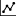
\includegraphics[width=0.5\textwidth]{img/sample/sample_png.png}
        \caption[sample image (png)]{sample image: when its extension is png.}
        \label{fig:sample_png}
    \end{figure}
    labelで指定することで, \figref{fig:sample_png}はxxxのように参照することができる.\\
    captionでは [] が目次に示される内容で, \{\} が本文に示される内容である. 同じでいい場合は \{\} のみで良い.\\
    上記のように, pngやjpegのようなラスタ画像を用いると, 拡大したときに荒くなってしまう.\\
    下記のようにpdfのようなベクタ画像を用いると拡大しても荒くならない.
    ただし, 保存時にベクタ形式にする必要がある.
    \begin{figure}[htbp]
        \centering   
        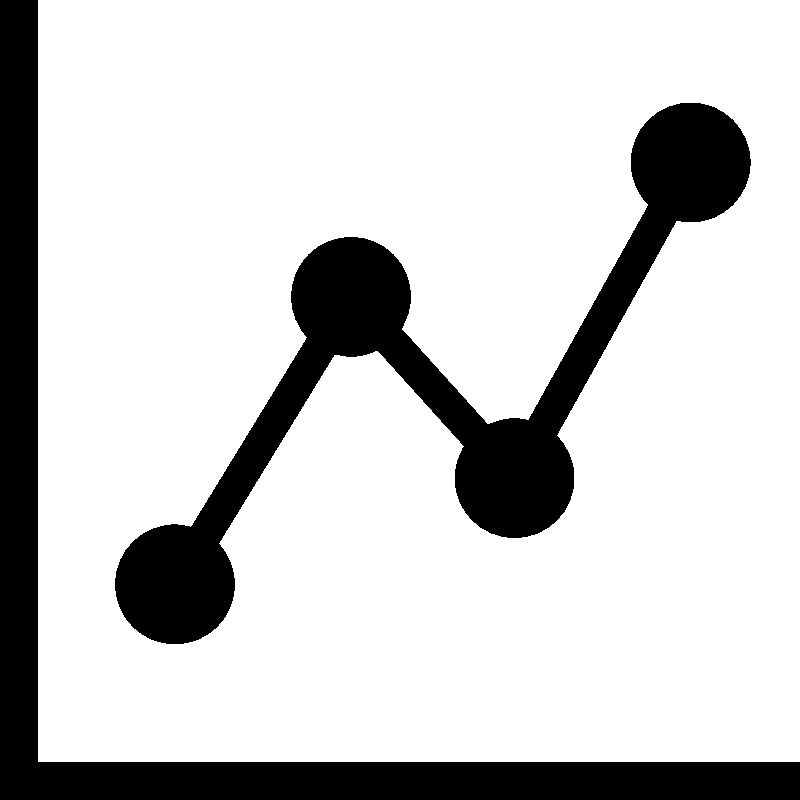
\includegraphics[width=0.5\textwidth]{img/sample/sample_pdf.pdf}
        \label{Fig:sample_pdf}
        \caption[sample image (pdf)]{sample image: when its extension is pdf.}
    \end{figure}
    出力の位置は[htbp]で指定するが, レイアウトによっては自動的に次のページに移動するなど, 指定した通りに配置できないときがある.\\
    この場合は[H]のように大文字で指定すると,
    \begin{figure}[H]
        \centering   
        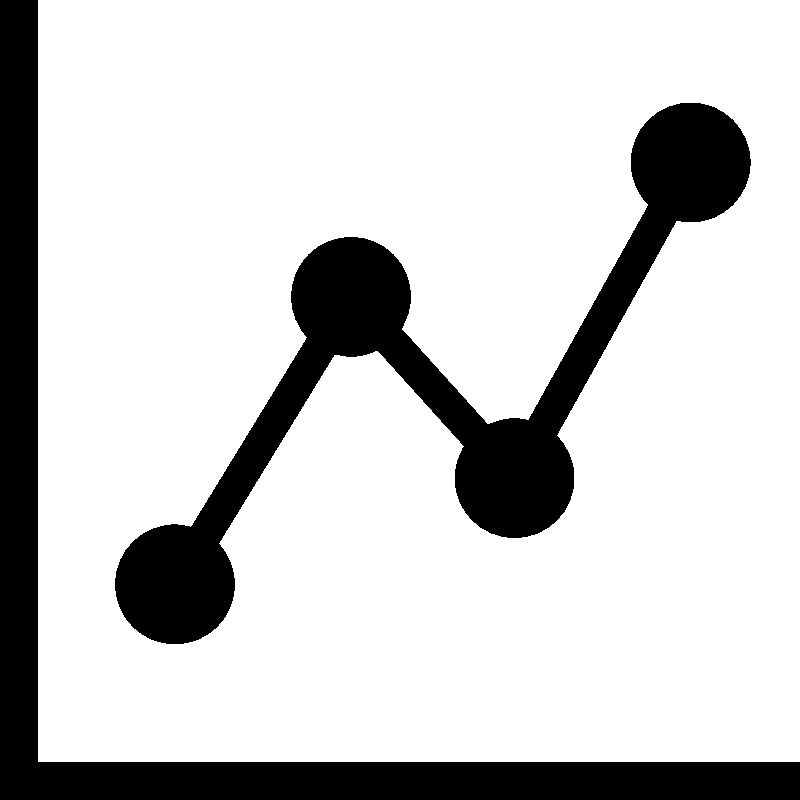
\includegraphics[width=0.5\textwidth]{img/sample/sample_pdf.pdf}
        \label{Fig:sample_pdf_here}
        \caption[sample image (pdf, here)]{sample image: when its extension is pdf and is enforced to be here.}
    \end{figure}
    このように強制的に配置が可能になる.

    \subsection{複数画像の挿入}
    複数画像の挿入方法はいくつかあるようだが, とりあえず下記で挿入することが可能.
    \begin{figure}[H]
		\centering
		\begin{tabular}{c}
		% ----- image 1 =====
			\begin{minipage}{0.25\hsize}
				\centering
				
\includegraphics[width=\textwidth]{img/sample/sample1.pdf}
				\text{(a)}
			\end{minipage}
		% ----- image 2 =====
			\begin{minipage}{0.25\hsize}
				\centering
				
\includegraphics[width=\textwidth]{img/sample/sample2.pdf}
				\text{(b)}
			\end{minipage}
		% ----- image 3 =====
			\begin{minipage}{0.25\hsize}
				\centering
				
\includegraphics[width=\textwidth]{img/sample/sample3.pdf}
				\text{(c)}
			\end{minipage}
		% ----- image 4 =====
			\begin{minipage}{0.25\hsize}
				\centering
				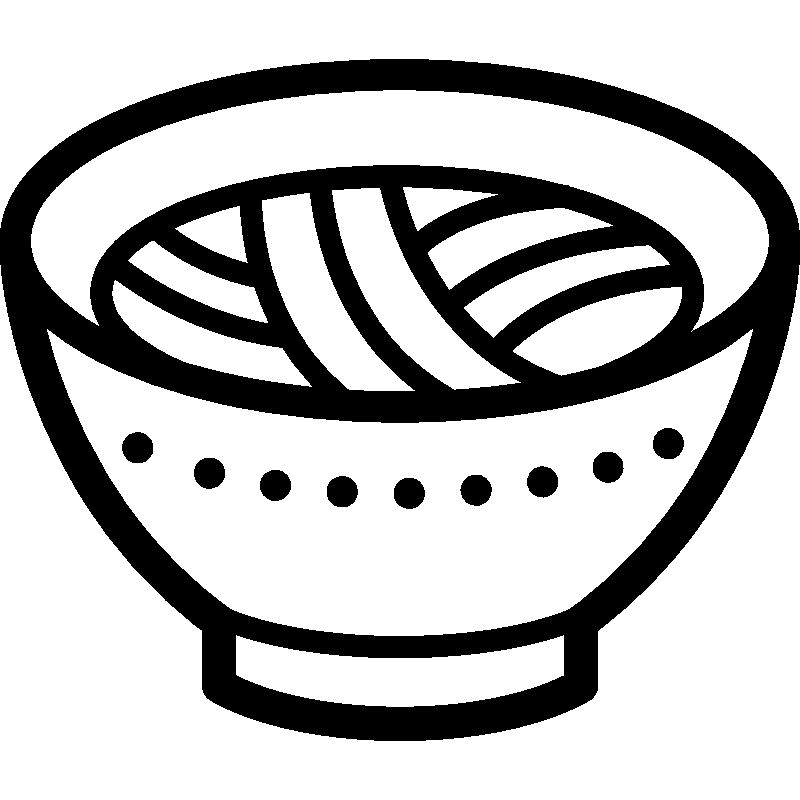
\includegraphics[width=\textwidth]{img/sample/sample4.pdf}
				\text{(d)}
			\end{minipage}
		\end{tabular}
		\caption[Four sample images]
		{
			Four sample images.
			(a) sushi (b) milk (c) peach (d) ramen
		}
		\label{fig:sample_four_images}
	\end{figure}

    縦2横2にすることも可能.
    \begin{figure}[H]
		\centering
		\begin{tabular}{c}
		% ----- image 1 =====
			\begin{minipage}{0.25\hsize}
				\centering
				
\includegraphics[width=\textwidth]{img/sample/sample1.pdf}
				\text{(a)}
			\end{minipage}
			\hspace{1cm}
		% ----- image 2 =====
			\begin{minipage}{0.25\hsize}
				\centering
				
\includegraphics[width=\textwidth]{img/sample/sample2.pdf}
				\text{(b)}
			\end{minipage}
			\vspace{1cm}\\
		% ----- image 3 =====
			\begin{minipage}{0.25\hsize}
				\centering
				
\includegraphics[width=\textwidth]{img/sample/sample3.pdf}
				\text{(c)}
			\end{minipage}
			\hspace{1cm}
		% ----- image 4 =====
			\begin{minipage}{0.25\hsize}
				\centering
				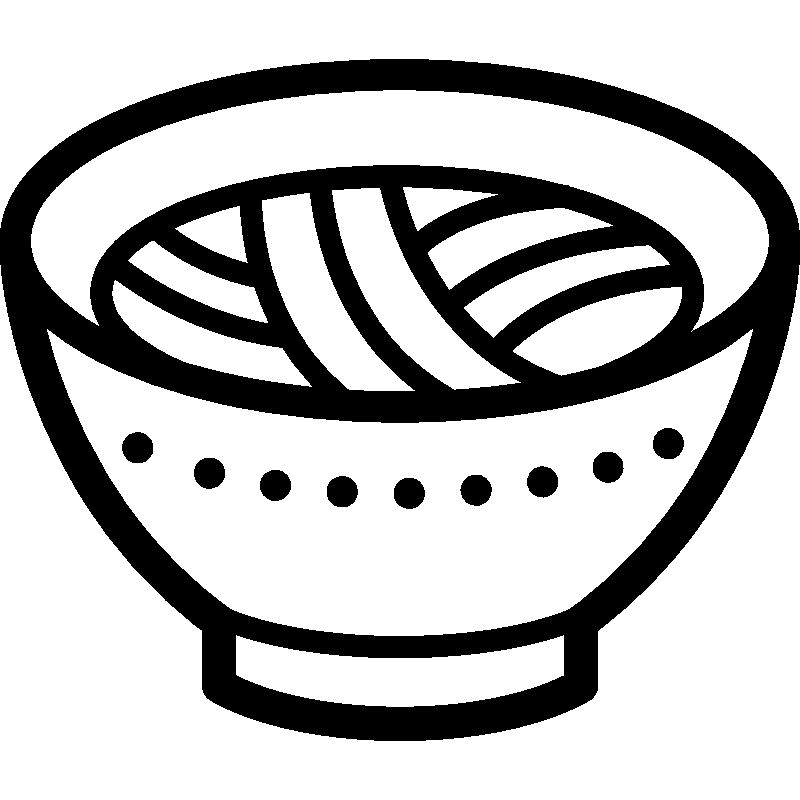
\includegraphics[width=\textwidth]{img/sample/sample4.pdf}
				\text{(d)}
			\end{minipage}
		\end{tabular}
		\caption[Four sample images]
		{
			Four sample images 2.
			(a) sushi (b) milk (c) peach (d) ramen
		}
		\label{fig:sample_four_images2}
	\end{figure}
    
\section{Table}
Tableは\tbref{tb:sample_table}のようにして挿入する.
\begin{table}[H]
	\centering
	\caption{Sample Table: accuracy for train/evaluation data.}
	\begin{tabular}{ll}\hline
		 訓練データの正答率&: $98\%$ \\
		 テストデータの正答率&: $88\%$ \\
	\label{tb:sample_table}
	\end{tabular}
\end{table}

\section{Bib}
参考文献は, \cite{author:06}とすれば良い.
複数の参考文献を扱う場合は, \cite{author:06, conference:06}のようにする.\\
使用してない参考文献は自動的に記載されないようになっているので, とりあえずbib/liter.bibに入れておいて構わない.\\
通し番号は本文で言及された順になるがこれも自動的に処理されるので気にしなくて良い.

\section{Equation}
数式の入力はたくさんある.
文章中であれば, $x = 2$ のように挿入できる.\\
数式環境を用意する場合は, \equref{eq:sample1}, \equref{eq:sample2}, \equref{eq:sample3}のようにできる.

\begin{align}
    x &= 2 \label{eq:sample1}\\
    y &= x^2 + 1 \label{eq:sample2}\\
      &= 5 \label{eq:sample3}
\end{align}


\begin{equation}\rho_0=(1−db)|vac\rangle\langle vac|+b
\sum_{k=1}^{d}|k\rangle\langle k| \label{sample_rho_0}
\end{equation}

\begin{equation}
\begin{split}
\rho_1&=(1−\eta)((1−db)|vac\rangle\langle vac|+bI)+\eta\rho\\
&=(1−\eta)(1−db)|vac\rangle\langle vac|+(1-\eta)bI+\eta\rho
\end{split} \label{sample_rho_1}
\end{equation}

\section{プログラム}
プログラムを掲載するには以下のようにする。

\begin{lstlisting}[caption=hoge,label=fuga]
# -*- coding: utf-8 -*-
import cmath
import math
import numpy
from scipy.stats import norm
import numpy as np
import numpy.linalg as LA
import matplotlib.pyplot as plt
\end{lstlisting}

\section{記号をそのまま出力}

\verb|abc_xy|
 % 使い方を示す例
\chapter{序論}

\section{本研究の目的と方法}
この論文では、情報理論における通信の基本的な扱い方を理解することを目標にする。
そのため、通信路行列についてまず説明し、次にエントロピー、相互情報量、通信容量について説明する。

\section{本論文の構成}
本論文は本章を含め, 6つの章と2つの付録からなる.
\begin{itemize}
	\item 第1章では本論文の位置づけについて記した.
	\item 第2章では通信路について記した.
	\item 第3章ではエントロピーと通信容量について記した.
	\item 第4章ではコヒーレント状態を用いた通信について記した.
	\item 第5章では減衰通信路を用いた通信について記した.
 	\item 第6章では結論を記した.
	\item 付録Aではその他の本研究に関する予備実験や補足事項について述べた.
	\item 付録Bではその他の実験を載せた.
\end{itemize}
\chapter{通信路}
まず、通信路について説明する。通信路に入力される記号$\{a_1,b_2,…,b_r\}$の集合$A_c$を入力アルファベットと呼ぶ。
また、通信路から出力される記号$\{b_1,b_2,…,b_r\}$の集合$A_r$を出力アルファベットと呼ぶ。

ここで、$a_i$が入力された時に$b_j$が出力される条件付き確率$P(b_j|a_i)$を要素とする行列を通信路行列と呼ぶ。
定常無記憶通信路の確率的性質は通信路行列
$$T=[p_{ij}],p_{ij}=P(b_j|a_i)$$ $$(i=1,2,\cdots ,q;j=1,2,\cdots,r)$$
で完全に表すことができる。



 通信路の例として、2元対称通信路について説明する。
2元対称通信路の通信路行列は以下のようにあらわすことができる。
$$
T=\begin{bmatrix}
1-p&p\\
p&1-p
\end{bmatrix}
(0≦p≦1)$$ 
これを通信路線図を用いて書くと\figref{Fig2_1}のように書くことができる。

    \begin{figure}[H]
        \centering   
        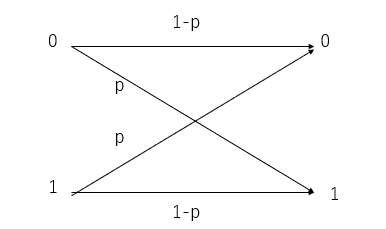
\includegraphics[width=0.7\textwidth]{img/Fig1.png}
        \caption[sample image (png)]{通信路線図}
        \label{Fig2_1}
    \end{figure}


ここで、$0$が入力されると確率 $1-p$で$0$が出力され、確率$p$で$1$が出力されることがわかる。
一方$1$が入力されると確率$p$で$0$が出力され、確率1-pで$1$が出力される。



\chapter{エントロピーと通信容量}
次に通信容量について説明する。
通信容量は、通信路で伝達できる最大の($1$記号当りの)情報量のことである。
通信容量$C$はこのようにして計算することができる。
$$
C=\max_{P_X}I(X;Y)
$$
ここで、$\max_{P_X}$は先験確率$P_X$を動かして最大値を求めることを意味している。
すなわち通信容量は相互情報量I(X;Y)を$P_X$で最大化したものとなっている。相互情報量は、出力$Y$を知ったときに得る$X$に関する情報量のことで、通信路で伝達される情報量を表している。



相互情報量について詳しく見るために、エントロピーについて説明をする。
エントロピーとはXに関する曖昧さを表す量で、このような式で計算することができる。
$$
H(X)=-\sum_xP_X(x)\log P_X(x)
$$
条件付きエントロピーは、
$Y$の値を知った時に$x$に関して残る平均の曖昧さを表す量で、
このような式で計算することができる。
$$
H(X|Y)=\sum_xP_Y(y)H(X|Y=y)$$
$$
H(X|Y=y)=-\sum_xP(x|y)\log P(X|Y)
$$




相互情報量は、エントロピーから条件付きエントロピーを引いたもののことでこのように表される。
$$
I(X;Y)=H(X)-H(X|Y)
$$
さきほど説明したように、エントロピー$H(X)$は、Xに関する曖昧さを表しており、
条件付きエントロピー$H(X|Y)$は、$Y$の値を知った時に$x$に関して残る平均の曖昧さ
を表している。したがって$H(X)$から$H(X|Y)$を引くとYの値を知ることにより、消えた$X$の曖昧さになる。
すなわちこれは、出力$Y$を知ったときに得る$X$に関する情報量となっている。
\figref{Fig3_1}は相互情報量とエントロピーの関係を表している。


    \begin{figure}[H]
        \centering   
        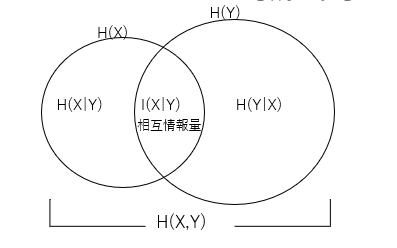
\includegraphics[width=0.7\textwidth]{img/Fig2.png}
        \caption[sample image (png)]{相互情報量とエントロピーの関係}
        \label{Fig3_1}
    \end{figure}


$H(X)$から$H(X|Y)$を引くと相互情報量$I(X|Y)$となるが、
$H(Y)$から$H(Y|X)$を引いても相互情報量$I(X|Y)$が得られることが知られている。


次に2元対称通信路の通信容量について計算する。
さきほど説明したように、通信容量は以下の式で計算することができる。
$$
C=\max_{P_X}I(X;Y)
$$
ここで、最適な$P_X$は、$P_X(0)=P_X(1)=1/2$となることが知られているので、
この事実を使って通信容量を計算することにする。
このとき、$P_Y(0)=P_Y(1)$を計算すると$1/2$となる。
また、エントロピー$H(Y)$は$1$となり、条件付きエントロピーは
$$
-p\log_2p-(1-p)\log_2(1-p)
$$
となる。
よって通信容量$C$はこのように$p$を使って計算できる。


\chapter{コヒーレント状態を用いた通信}
次にコヒーレント状態を用いた通信について考える。
複素振幅αを持つ光の状態をコヒーレント状態と呼ぶ。コヒーレント状態$\alpha$は以下のような式で与えることができる。

\begin{equation}
|\alpha\rangle=\sum_nC_n|n\rangle
\end{equation}


ここでは、$\alpha$を実数として、コヒーレント状態 $\alpha$、$-\alpha$を用いて通信について考える。

この通信では、$0$に対して$-\alpha$を、$1$に対して$\alpha$を送信する。
受信者はホモダイン測定を行い、その測定値に対してしきい値処理をおこなって$0$または$1$出力する。


ホモダイン測定では、コヒーレント状態の複素振幅$\alpha=x+iy$の$x$成分を測定する。

    \begin{figure}[H]
        \centering   
        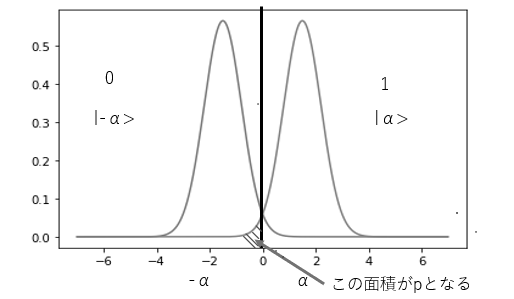
\includegraphics[width=1\textwidth]{img/Fig3.png}
        \caption[sample image (png)]{コヒーレント状態をホモダイン測定した場合の出力の確率分布}
        \label{Fig4_1}
    \end{figure}




\figref{Fig4_1}は、コヒーレント状態$\alpha$と$-\alpha$の測定値の確率分布のグラフを表している。この分布はそれぞれ分散$1/4$の正規分布となっている。
そして、閾値を$0$に設定し測定値が$0$より小さい場合は$0$、大きい場合は$1$を受信したと判断する。
したがって、この通信路は2元対称通信路となり、この面積が誤り確率$p$を表している。
したがって、この面積を計算すると通信容量を求めることが可能になる。


誤り確率$p$は、以下のような積分によって計算することができる。
$$
\int_{-\infty}^{x_0}f(x)dx
$$この積分は累積分布関数を用いて計算することができる。
累積分布関数はPythonを用いると以下のように書くことによって計算することができる。

\begin{lstlisting}[caption=累積分布関数]
p=norm.cdf(0,loc=x,scale=0.25)
\end{lstlisting}

また、通信容量は以下のように書いて計算することができる。

\begin{lstlisting}[caption=通信容量]
C=1+p*np.log(p)+(1-p)*np.log(1-p)
\end{lstlisting}


    \begin{figure}[H]
        \centering   
        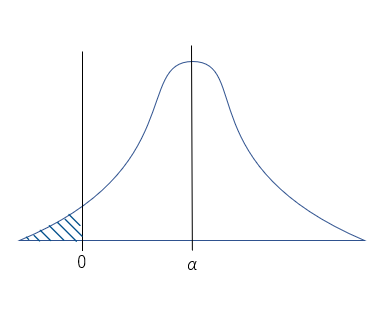
\includegraphics[width=0.7\textwidth]{img/Fig4.png}
         \caption[sample image (png)]{正規分布}
        \label{Fig4_2}
    \end{figure}

\figref{Fig4_2}はコヒーレント状態$|x\rangle$の測定値の確率分布のグラフをわかりやすくしたものである。


\begin{lstlisting}[caption=αの変化で変わる通信容量]
x=np.arange(0,5,0.01)
p=norm.cdf(0,loc=x,scale=0.25)
c=1+p*np.log(p)+(1-p)*np.log(1-p)
plt.plot(x,c)
\end{lstlisting}
\figref{Fig4_3}は、通信容量の計算の結果である。
信号$\alpha$と$-\alpha$を区別することが容易となるので誤り率$p$はほとんど$0$となる。
そのため\figref{Fig4_3}において、$\alpha$の値が大きくなると、通信容量$1$に近づいている。

    \begin{figure}[H]
        \centering   
        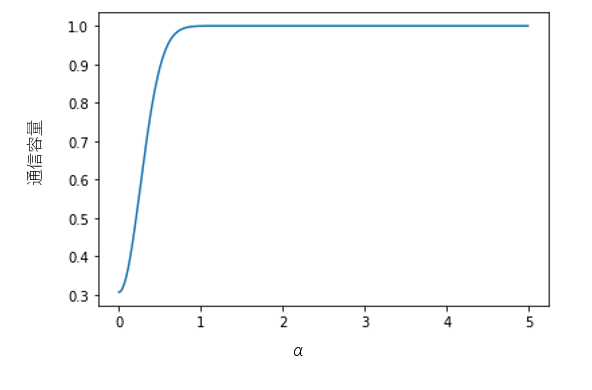
\includegraphics[width=0.7\textwidth]{img/Fig5.png}
        \caption[sample image (png)]{$\alpha$の変化で変わる通信容量}
        \label{Fig4_3}
    \end{figure}
。
    

\chapter{減衰通信路を用いた通信}
減衰通信路を用いた通信を行う場合の通信容量を計算する。
以下は通信容量のグラフを書くためのプログラムである。

\begin{lstlisting}[caption=減衰通信路の通信容量,label=program5_1]
import japanize_matplotlib
x=np.arange(0,5,0.01)
y1=[]
arate=0.05 #@param {type: "number"}
for x_val in x:
  q_state=Qstate(x_val)
  q_state.attenuate(arate)
  p=norm.cdf(0,loc=q_state.alpha,scale=np.sqrt(q_state.a[0][0]))
  c=1+p*np.log(p)+(1-p)*np.log(1-p)
  y1.append(c)
y2=[]
for x_val in x:
  q_state=Qstate(x_val)
  q_state.attenuate(np.sqrt(arate))
  q_state.amplificate(1/np.sqrt(arate))
  q_state.attenuate(np.sqrt(arate))
  p=norm.cdf(0,loc=q_state.alpha,scale=np.sqrt(q_state.a[0][0]))
  c=1+p*np.log(p)+(1-p)*np.log(1-p)
  y2.append(c)

plt.plot(x,y1,label="増幅器なし",c="black",ls="dotted")
plt.plot(x,y2,label="増幅器あり",c="black",ls="-")
plt.legend()
plt.show()
\end{lstlisting}

\figref{Fig5_1}は、透過率$\lambda=0.05$の時の通信容量のグラフを表している。実線は増幅器ありの場合、点線は増幅器なしの場合のグラフである。グラフの横軸は信号の振幅値を表し、縦軸は通信容量を表している。グラフより、透過率$\lambda=0.05$の場合は、増幅器を設置することにより、通信容量を大きくする効果があることがわかる。

    \begin{figure}[H]
        \centering   
        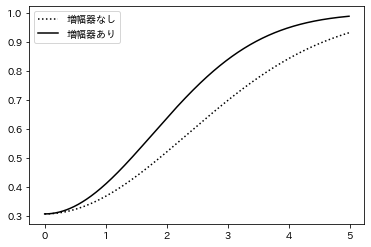
\includegraphics[width=1\textwidth]{img/Fig5_1.png}
        \caption[sample image (png)]{$\lambda=0.05$のときの通信容量の変化}
        \label{Fig5_1}
    \end{figure}

\newpage
\figref{Fig5_2}は、透過率$\lambda=0.1$の時の通信容量のグラフを表している。実線は増幅器ありの場合、点線は増幅器なしの場合のグラフである。グラフの横軸は信号の振幅値を表し、縦軸は通信容量を表している。グラフより、透過率$\lambda=0.1$の場合は、増幅器を設置することにより、通信容量は大きいが、$\lambda=0.05$の時よりほどではないことがわかる。

    \begin{figure}[H]
        \centering   
        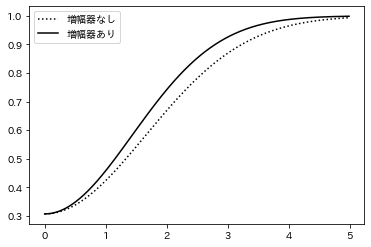
\includegraphics[width=1\textwidth]{img/Fig5_2.png}
        \caption[sample image (png)]{$\lambda=0.1$のときの通信容量の変化}
        \label{Fig5_2}
    \end{figure}


\newpage
\figref{Fig5_3}は、透過率$\lambda=0.2$の時の通信容量のグラフを表している。実線は増幅器ありの場合、点線は増幅器なしの場合のグラフである。グラフの横軸は信号の振幅値を表し、縦軸は通信容量を表している。グラフより、透過率$\lambda=0.2$の場合は、増幅器を設置していても通信容量はほぼ変わらないことがわかる。

    \begin{figure}[H]
        \centering   
        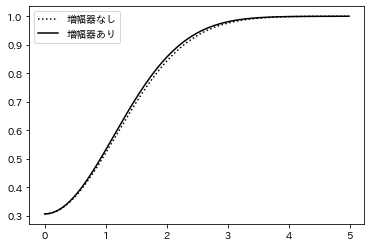
\includegraphics[width=1\textwidth]{img/Fig5_3.png}
        \caption[sample image (png)]{$\lambda=0.2$のときの通信容量の変化}
        \label{Fig5_3}
    \end{figure}


\newpage
\figref{Fig5_4}は、透過率$\lambda=0.3$の時の通信容量のグラフを表している。実線は増幅器ありの場合、点線は増幅器なしの場合のグラフである。グラフの横軸は信号の振幅値を表し、縦軸は通信容量を表している。グラフより、透過率$\lambda=0.3$の場合も増幅器を設置していても通信容量はほぼ変わらないことがわかる。

    \begin{figure}[H]
        \centering   
        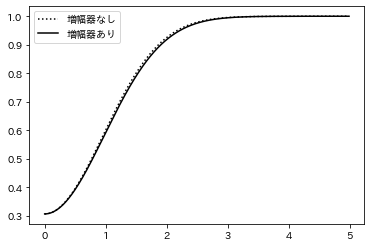
\includegraphics[width=1\textwidth]{img/Fig5_4.png}
        \caption[sample image (png)]{$\lambda=0.3$のときの通信容量の変化}
        \label{Fig5_4}
    \end{figure}

\newpage
\figref{Fig5_5}は、透過率$\lambda=0.6$の時の通信容量のグラフを表している。実線は増幅器ありの場合、点線は増幅器なしの場合のグラフである。グラフの横軸は信号の振幅値を表し、縦軸は通信容量を表している。グラフより、透過率$\lambda=0.6$の場合も増幅器を設置していても通信容量はほぼ変わらないことがわかる。

    \begin{figure}[H]
        \centering   
        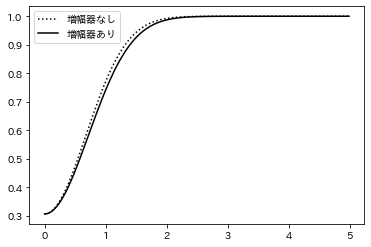
\includegraphics[width=1\textwidth]{img/Fig5_5.png}
        \caption[sample image (png)]{$\lambda=0.6$のときの通信容量の変化}
        \label{Fig5_5}
    \end{figure}


\newpage
\figref{Fig5_6}は、透過率$\lambda=0.9$の時の通信容量のグラフを表している。実線は増幅器ありの場合、点線は増幅器なしの場合のグラフである。グラフの横軸は信号の振幅値を表し、縦軸は通信容量を表している。グラフより、透過率$\lambda=0.9$の場合も増幅器を設置していても通信容量はほぼ変わらないことがわかる。

    \begin{figure}[H]
        \centering   
        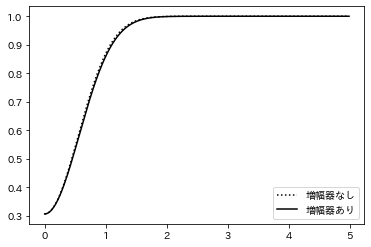
\includegraphics[width=1\textwidth]{img/Fig5_6.png}
        \caption[sample image (png)]{$\lambda=0.9$のときの通信容量の変化}
        \label{Fig5_6}
    \end{figure}






    

\chapter{結論}
今回の研究で、減衰通信路を用いた通信を行った。その結果、透過率を上げていくにつれ、増幅器を使用しても通信容量がほぼ変化しない部分があることに気づいた。また、透過率をそれ以上上げても通信容量がほぼ変化しないことにも気づいた。
%\chapter*{謝辞}
\addcontentsline{toc}{chapter}{謝辞}

本研究は, 東京大学 大学院 情報理工学系研究科 知能機械情報学専攻 your professor 教授のご指導のもとで行われました.
%\bibliographystyle{bib/IEEEtransBST/IEEEtran}
\bibliography{bib/style,bib/liter}

\renewcommand{\prechaptername}{付録}
\renewcommand{\postchaptername}{}
\renewcommand{\thechapter}{\Alph{chapter}}
\setcounter{chapter}{0}

\chapter{量子状態のクラスのプログラム}
\begin{lstlisting}[caption=量子状態のクラス,label=Qstate]
# -*- coding: utf-8 -*-
import cmath
import math
import numpy
from scipy.stats import norm
import numpy as np
import numpy.linalg as LA
import matplotlib.pyplot as plt

#振幅値 
A = 1.0
#行列Jを指定
J = np.array([[0, 1] , [-1, 0]])
#単位行列Iを指定
Id = np.array([[1.0, 0] , [0 , 1.0]])  

class Qstate:
    """量子ガウス状態を表すクラス"""
    def __init__(self, c_amplitude = A + 0j ):
        """初期値の設定を追加 (sohma Aug 12 2018)"""
        # 複素振幅値
        self.alpha = c_amplitude

        # コヒーレント状態の正規分布の広がり(共分散行列)を表す        
        self.a = np.array([[0.25 , 0] , [0 , 0.25]])

        # 正規受信者の確率        
        self.Pr = 0.0
        
        
    def attenuate(self, att_rate):
        """減衰する
           aの値(共分散)と平均が変換される"""
        #減衰後の複素振幅を計算
        self.alpha = self.alpha* math.sqrt(att_rate)
        #減衰後の共分散行列を計算
        self.a = (att_rate * self.a) + ((1.0-att_rate) * Id / 4.0)

    def amplificate(self,gain):
        """増幅する
           aの値(共分散)と平均が変換される"""
        #増幅後の複素振幅を計算
        self.alpha =  self.alpha* math.sqrt(gain)
        #増幅後の共分散行列を計算
        self.a = (gain * self.a) + ((gain-1.0) * Id / 4.0)


    def measure_homodyne(self, theta_val):
        """ホモダイン測定を行う"""     
        # 量子状態を元の位置まで回転させる
        rev_rot =  cmath.rect(1.0, theta_val)
        beta =  self.alpha * rev_rot
        U = np.array([[math.cos(theta_val) , -math.sin(theta_val)] , [math.sin(theta_val) , math.cos(theta_val)]])
        b = np.dot(U.T , np.dot(self.a , U))
        
        # 共分散行列 b の x軸方向の標準偏差
        dev_x = math.sqrt(b[0, 0])
        
        # 0が出力される確率(測定値が正になる確率)       
        self.Pr =  norm.sf(x = 0.0 , loc = beta.real ,scale = dev_x )
        return self.Pr
    
    def homodyne_measurement(self):
        dev_x=math.sqrt(self.a[0,0])
        res = np.random.normal(loc=np.real(self.alpha), scale = dev_x)
        return res

    def plot_distribution(self,ax,max_x,max_y,min_x,min_y,c_name="blue"):  
      x = np.arange(min_x, max_x, 0.01) # x点として[min_x, max_y]まで0.01刻みでサンプル
      y = np.arange(min_y, max_y, 0.01)  # y点として[min_x, max_y]まで0.01刻みでサンプル
      x, y = np.meshgrid(x, y)  # 上述のサンプリング点(x,y)を使ったメッシュ生成
      dev_x=math.sqrt(self.a[0,0])   #共分散行列を表す属性a[0,0]の平方根をdev_xに代入
      dev_y=math.sqrt(self.a[1,1])   #共分散行列を表す属性a[1,1]の平方根をdev_yに代入
      z = norm.pdf(x,self.alpha.real,dev_x)*norm.pdf(y,self.alpha.imag,dev_y)
      ax.set_zlim(0.0,1.0)
      ax.plot_wireframe(x, y, z, color=c_name,linewidth=0.3) # ワイヤーフレームのプロット。color,linewidthは曲面のメッシュの線の色と太さをそれぞれ表す。

      ax.tick_params(labelbottom="off",bottom="off") # x軸の削除
      ax.tick_params(labelleft="off",left="off") # y軸の削除
      #ax.set_xticklabels([]) 
      #ax.set_yticklabels([])
      ax.set_zticklabels([])

    def homodyne(self,thld):#arrがthld(しきい値)より大きければ1,小さければ0を出力する
      arr=np.random.normal(self.alpha.real,np.sqrt(self.a[0][0]),1) #平均self.alpha.real,標準偏差np.sqrt(self.a[0][0]),乱数を1個出力する正規分布をarrに代入
      #print("arr:",arr,"thld:",thld)
      if arr>thld:
        return 1
      else:
        return 0
         #1か0を出力する
\end{lstlisting}






%\renewcommand{\prechaptername}{付録}
\renewcommand{\postchaptername}{}
\renewcommand{\thechapter}{\Alph{chapter}}

\chapter{その他の実験}

% 後書き
\backmatter
\appendix

\printindex
\end{document}